\documentclass[main.tex]{subfiles}

\begin{document}
In sintesi, i modelli proposti nell'analisi hanno la seguente capacità predittiva:
\begin{figure}[H]
	\centering
	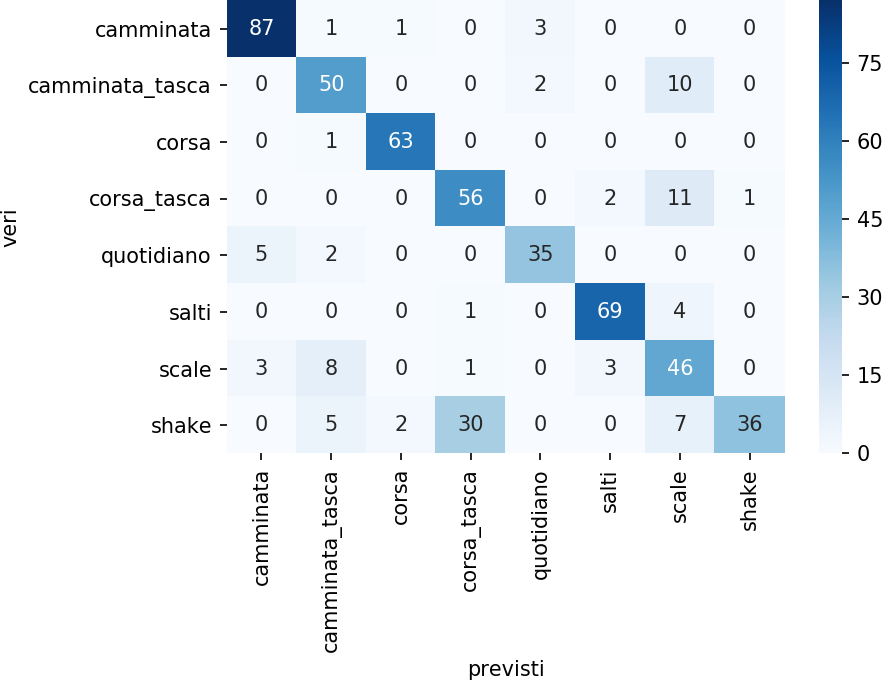
\includegraphics[width=.5\textwidth]{../../figure/confusionMatrix-Mn-test.png}
	\caption{Matrice di confusione ottenuta con il modello multinomiale nell'insieme di test.}
	\label{fig:mn}
\end{figure}

\begin{figure}[H]
	\centering
	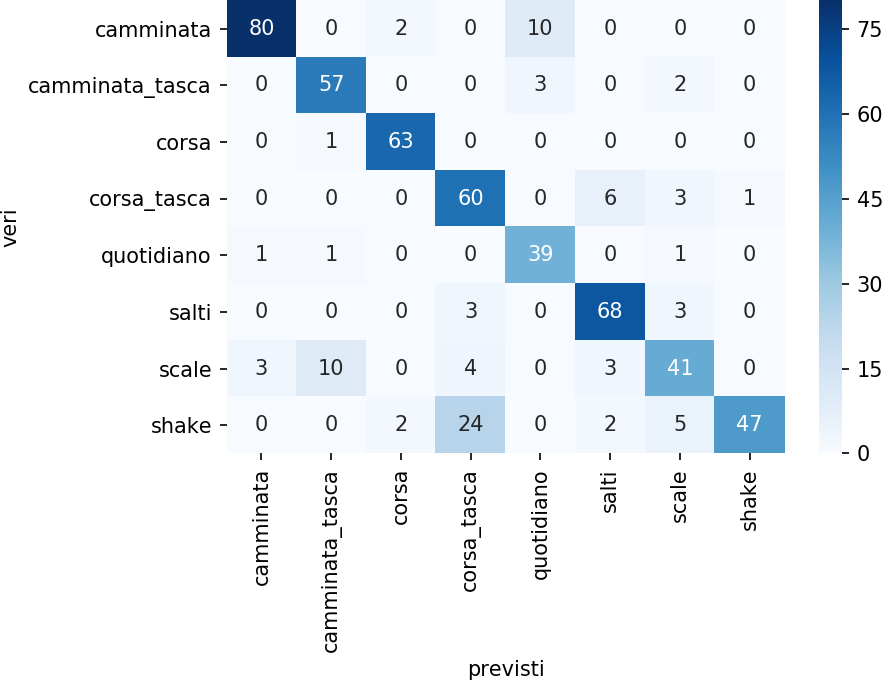
\includegraphics[width=.5\textwidth]{../../figure/confusionMatrix-QDA-penalizzata-test.png}
	\caption{Matrice di confusione ottenuta con la QDA pesata nell'insieme di test.}
	\label{fig:mn}
\end{figure}

\end{document}